%% ---------------------------------------------------------------------------
%% Controlling closed-book epistemic (un)certainty: BLADE vs.\ ITI on two models
%% ---------------------------------------------------------------------------

\begin{figure*}[t]
  \centering
  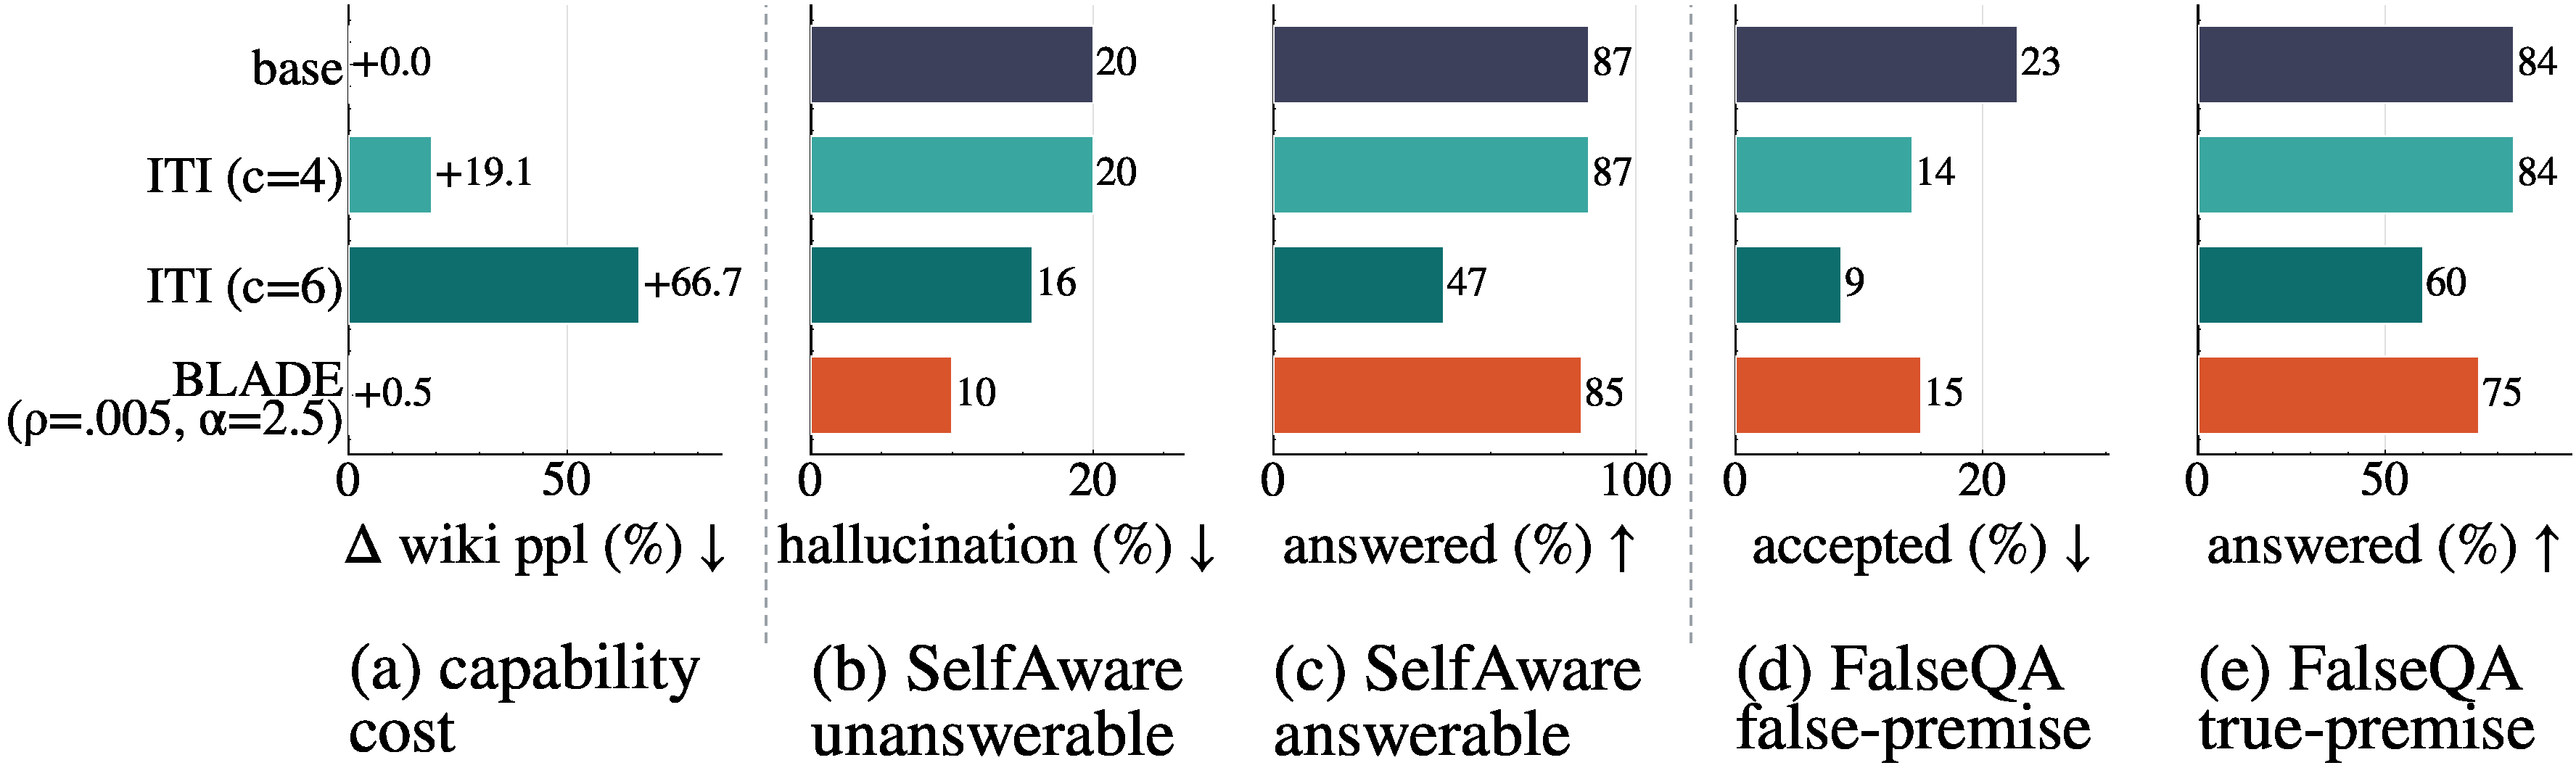
\includegraphics[width=\textwidth]{figures/uncertainty_method_cmp.pdf}
  \caption{\textbf{Controlling closed-book epistemic (un)certainty on Qwen3-8B.}
    A single BLADE weight edit ($\rho\!=\!0.005$, $\alpha\!=\!2.5$) vs.\ ITI
    activation steering~\citep{li2023iti} at two doses ($c\!=\!4,6$). Behavioral
    rates from a blind LLM judge; lower is better in (a,\,b,\,d), higher in (c,\,e).}
  \label{fig:uncertainty-method-cmp}
\end{figure*}

\begin{figure*}[t]
  \centering
  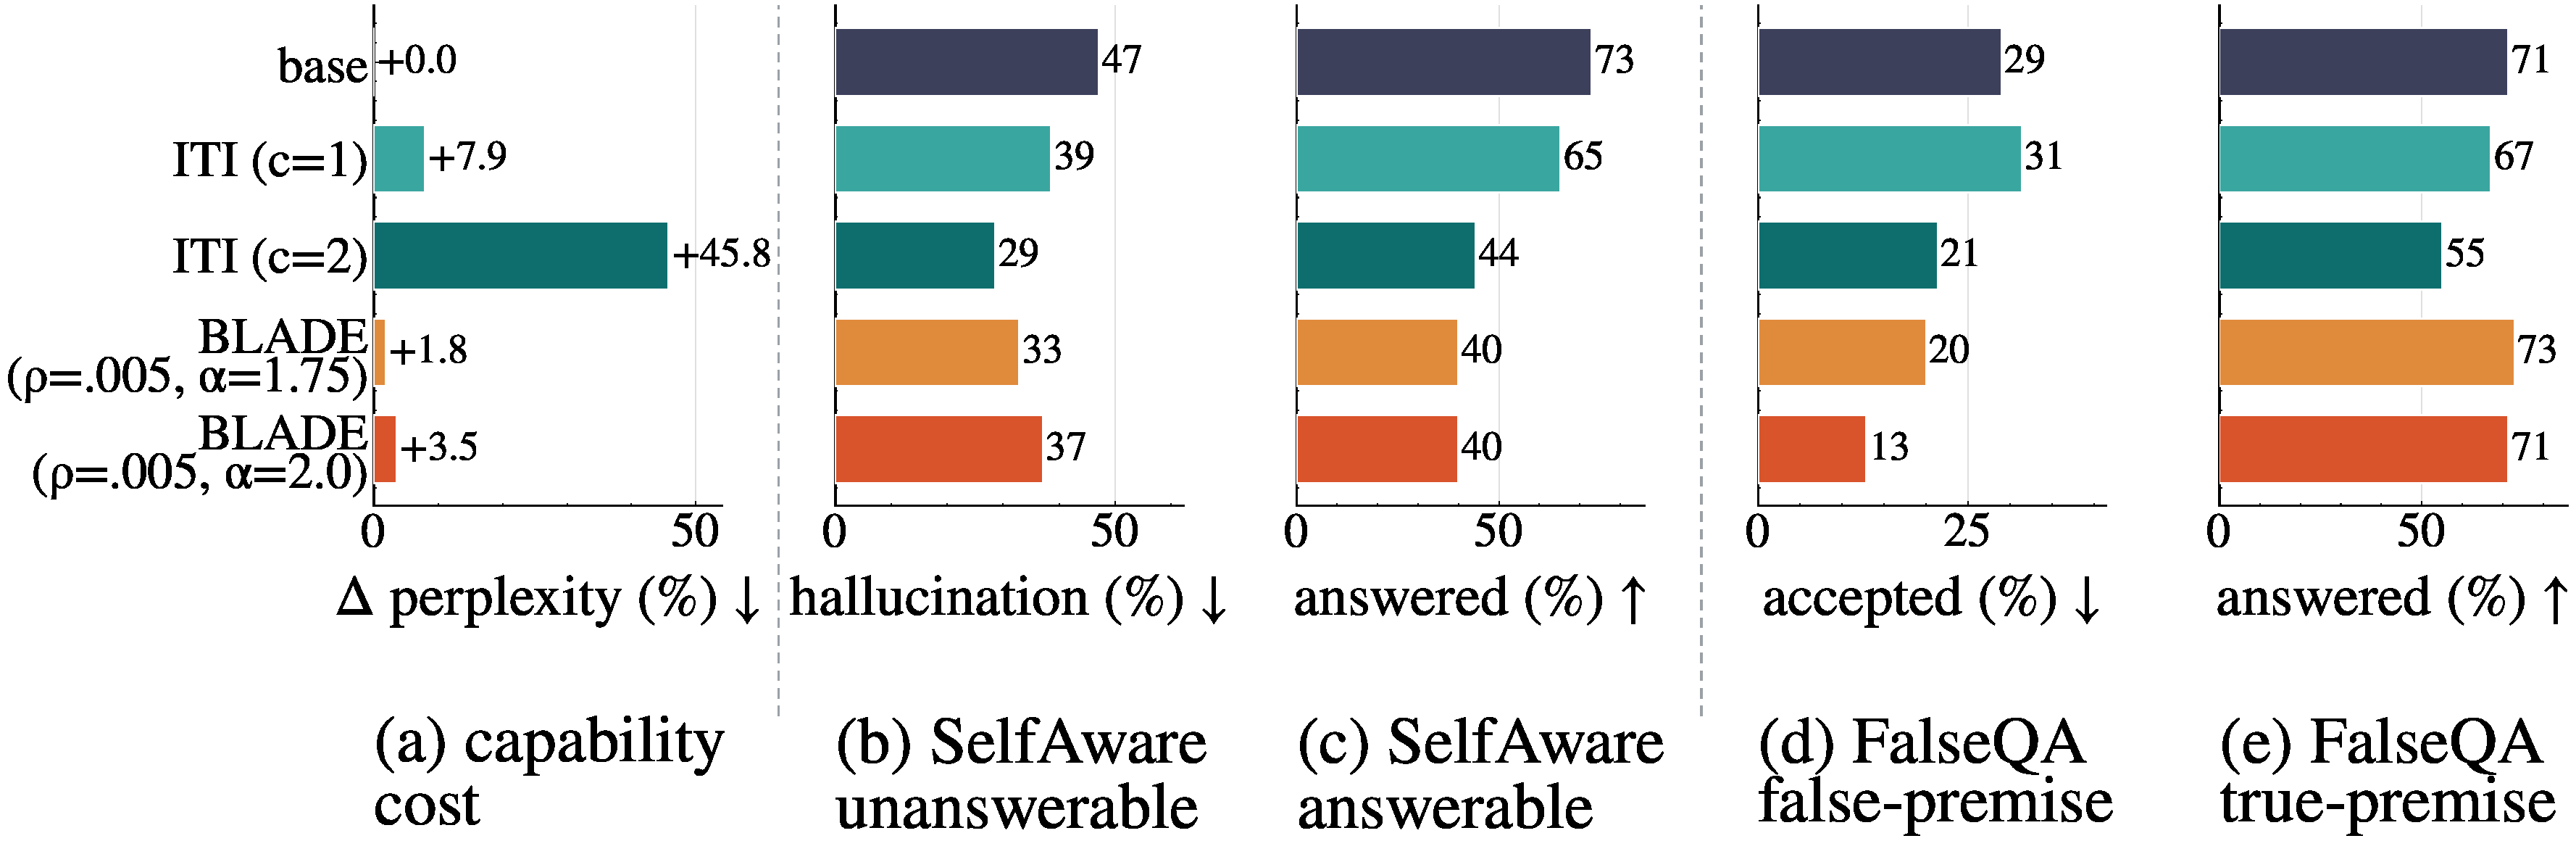
\includegraphics[width=\textwidth]{figures/uncertainty_method_cmp_llama.pdf}
  \caption{\textbf{Cross-model transfer to Llama-3.2-3B-Instruct.}
    Same layout and judge as Fig.~\ref{fig:uncertainty-method-cmp}, with doses
    re-swept for the smaller model: BLADE ($\rho\!=\!0.005$,
    $\alpha\!\in\!\{1.75,2.0\}$) vs.\ ITI~\citep{li2023iti} ($c\!\in\!\{1,2\}$).
    SelfAware/FalseQA use $n\!=\!70$ prompts per split.}
  \label{fig:uncertainty-method-cmp-llama}
\end{figure*}

\paragraph{Benchmarks.}
We evaluate on two closed-book abstention benchmarks, each of which pairs a
target failure with a matched behavior that a good intervention must preserve.
SelfAware~\citep{selfaware} pairs \emph{unanswerable} questions, on which the
model should abstain rather than hallucinate, with \emph{answerable} ones, on
which it should still answer. FalseQA~\citep{falseqa} pairs \emph{false-premise}
questions, on which the model should reject the premise rather than accept it,
with \emph{valid-premise} counterparts that it should answer normally. A blind
LLM judge (condition hidden) assigns every behavioral label. Capability cost is
the teacher-forced held-out WikiText perplexity change relative to the base model (BLADE-G's
generic-importance term is calibrated on C4, so WikiText is the held-out capability metric). Panels
(a,\,b,\,d) are lower-is-better; (c,\,e) are higher-is-better.

\paragraph{Setup.}
Both methods are fit on the \emph{same} certain-vs.-uncertain prompt contrast,
read at the last prompt token, so the comparison isolates the mechanism rather
than the direction source: BLADE compiles the contrast into a sparse static
weight edit (the BLADE-G variant, thinking-off, layers selected automatically by
ELS) with an amplification knob $\alpha$ and sparsity $\rho$, whereas
ITI~\citep{li2023iti} adds a per-head activation offset at inference time with a
dose $c$ measured in units of the per-head projection standard deviation. We
stress that $c$ and $\alpha$ are distinct knobs on distinct mechanisms; we sweep
each independently and compare the resulting operating points, not the
scalars themselves.

\paragraph{Qwen3-8B: a clean capability--behavior win.}
Figure~\ref{fig:uncertainty-method-cmp} shows that BLADE is the only
configuration that lowers SelfAware-unanswerable hallucination
(\ref{fig:uncertainty-method-cmp}b, $20\%\!\to\!10\%$) while leaving
perplexity flat ($+0.5\%$, \ref{fig:uncertainty-method-cmp}a) and answerable
questions answered ($85\%$ vs.\ $87\%$ base,
\ref{fig:uncertainty-method-cmp}c). ITI at $c\!=\!4$ costs $+19.1\%$
perplexity and does not move the unanswerable rate at all ($20\%$); only at
$c\!=\!6$ does it reach $16\%$, and it does so by inflating perplexity by
$+66.7\%$ and collapsing answerable-question answering from $87\%$ to $47\%$.
On FalseQA the two are closer: BLADE reduces false-premise acceptance from
$23\%$ to $15\%$ while holding valid-premise answering at $75\%$
(\ref{fig:uncertainty-method-cmp}d,\,e), and ITI reaches $14\%$ at $c\!=\!4$
with answering intact ($84\%$) but only $9\%$ at $c\!=\!6$, where answering
falls to $60\%$ alongside the capability collapse above. The distinguishing
axis is therefore SelfAware-unanswerable hallucination: BLADE removes it at no
measurable capability cost, and ITI cannot reach it without breaking the
model.

\paragraph{Llama-3.2-3B-Instruct: partial transfer on a harder testbed.}
Figure~\ref{fig:uncertainty-method-cmp-llama} repeats the comparison on a
smaller model, and the summary is that the Qwen operating point does
\emph{not} transfer as-is. Both interventions over-steer at Qwen strength, so we
swept lower doses (BLADE $\alpha\!\in\!\{1.75,2.0\}$, ITI
$c\!\in\!\{1,2\}$; $\rho$ fixed at $0.005$ throughout); each model evidently
needs its own $\alpha$ (and possibly $\rho$, untested here) and its own $c$. On SelfAware neither method finds a clean point: BLADE lowers
unanswerable hallucination from $47\%$ to $33\%$/$37\%$
(\ref{fig:uncertainty-method-cmp-llama}b), but answerable-question answering
drops from $73\%$ to $40\%$ (\ref{fig:uncertainty-method-cmp-llama}c), and
ITI traces the same steep trade-off ($39\%$/$29\%$ hallucination against
$65\%$/$44\%$ answering). We also note that the unanswerable rate is quantized
at $1/70$ granularity here, so single-case differences fall within sampling
noise, which makes FalseQA the more stable axis on this model. On that axis BLADE's characteristic signature survives: at
$\alpha\!=\!2.0$ it cuts false-premise acceptance from $29\%$ to $13\%$
(\ref{fig:uncertainty-method-cmp-llama}d) while fully preserving
valid-premise answering ($71\%$, identical to base,
\ref{fig:uncertainty-method-cmp-llama}e), at $+3.5\%$ perplexity
($+1.8\%$ at $\alpha\!=\!1.75$). ITI never matches this: at the mild $c\!=\!1$ it
actually \emph{raises} false-premise acceptance above base ($29\%\!\to\!31\%$) at
$+7.9\%$ perplexity, and at $c\!=\!2$ it reaches only $21\%$ acceptance while
cratering valid-premise answering to $55\%$ at $+45.8\%$ perplexity; its capability collapse arrives even earlier here than on Qwen
($c\!=\!2$ vs.\ $c\!=\!6$), suggesting the dose in per-head-std units is
miscalibrated for this model rather than merely too large. We omit SimpleQA
panels for Llama because its base already abstains on short fact-seeking
questions (roughly $1.5\%$ incorrect), leaving no hallucination headroom to
remove.

\paragraph{Cross-model reading.}
Taken together, the two figures locate where BLADE's advantage lives. On
Qwen3-8B, a model with genuine hallucination headroom that tolerates the edit,
BLADE yields a near-Pareto improvement: large gains on the target failures and
capability, at the cost of only $2$--$9$ percentage points on the matched
preserve-behaviors ($87\%\!\to\!85\%$ answerable, $84\%\!\to\!75\%$
valid-premise), and it is cheaper than ITI on capability and dominant on the
SelfAware axis. On Llama-3.2-3B the picture is messier:
the exact operating point fails to transfer, and on the noisier SelfAware
benchmark neither method separates the target failure from the matched
behavior. Yet on the more stable FalseQA axis BLADE still does what it did on
Qwen, removing the targeted failure (false-premise acceptance) at modest
capability cost ($+1.8$--$3.5\%$ perplexity) while leaving the matched
valid-premise behavior untouched, a
combination ITI does not reach without collapsing capability. We therefore
read the cross-model result as follows: BLADE's advantage (cheap, targeted,
answering-preserving) holds where the model has headroom, and holds partially
across models on the benchmark axis that is stable enough to measure it.
